\documentclass[dvipdfmx, 
				border = {5pt, 5pt, 5pt, 5pt}]{standalone}	% borderで余白をあける

\usepackage{bm}
\usepackage{tikz}	% ティクス

\usetikzlibrary{calc, angles, quotes}
\usetikzlibrary{intersections, math, patterns}
% intersections .. 交点の座標を求めるため
% math .. 計算を行う
% patterns .. 領域をパターンで塗りつぶすため

\begin{document}

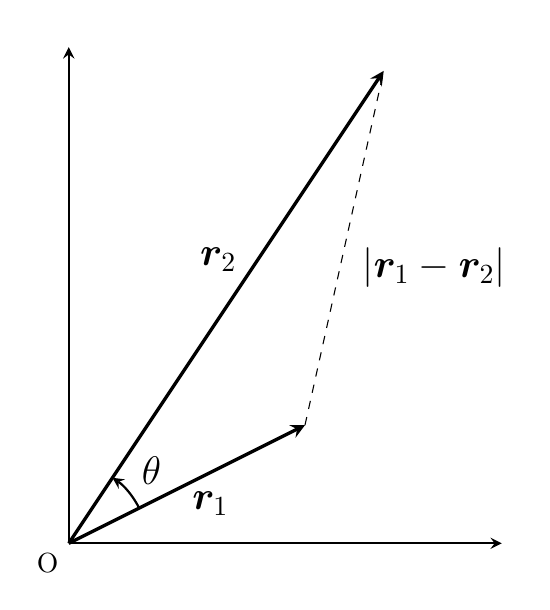
\begin{tikzpicture}[domain = -1.5:4, samples = 100, thick]	% sampleじゃなくてsamples
  \draw (0, 0) node[below left]{O};		% 原点

  % 斜線を引く
   %\fill [top color = white, bottom color = white, middle color = purple]
	% plot[sample = 100, domain = 0:4] (\x, {\x / 2 + 2})
	%(4, 4)--(4, 0)--(1, 0)--(0, 1) --(0, 2) -- (4, 4);

  % 斜線を引く
  % \fill [pattern = north east lines, very thin]		% 薄くしたいんだが
  %	% plot[sample = 100, domain = 0:4] (\x, {\x / 2 + 2})
  %	(4, 4)--(4, 0)--(1, 0)--(0, 1) --(0, 2) -- (4, 4);

  % 軸の描画
  \draw [thick, -stealth] (0, 0)--(5.5, 0) node[right] {$$};		% x軸
  \draw [thick, -stealth] (0, 0)--(0, 6.3) node[above] {$$};		% y軸


  % ベクトル
  \draw [very thick, -stealth] (0, 0)--(3, 1.5);
  \draw [very thick, -stealth] (0, 0)--(4, 6);
  
  % 点線
  \draw [thin, dashed] (3, 1.5)--(4, 6);

  \draw (1.8, 0.5) node {\Large $\bm{r}_1$};
  \draw (1.9, 3.6) node {\Large $\bm{r}_2$};
  \draw [right] (3.6, 3.5) node {\Large  $ |\bm{r}_1 - \bm{r}_2|$};
  
  % 角度
  \coordinate (O) at (0, 0);
  \coordinate (r1) at (3, 1.5);
  \coordinate (r2) at (4, 6);
  \draw  pic["\Large $\theta$",draw, -stealth, thick, angle eccentricity=1.4, angle radius=1cm] 
		{angle=r1--O--r2};	


  

  % 関数の描画
  % \draw [domain = -1.2:2] plot(\x, {-\x + 1}) 
  % 	node [right, fill = white, inner sep = 0pt]  at(2.1, -0.9) {$x_1 + x_2 = 1$};

  
  % 領域D
  % \draw (2.1, 1.5) node [fill = white] {$D$};

  % 座標
  % \node [below left] at(1, 0) {1};
  % \node [left] at(0, 1) {1}; 
  % \node [above left] at(0, 2) {2};		% left above ではだめ

\end{tikzpicture}

\end{document}
